\documentclass{article}
\usepackage{amsmath}
\usepackage{graphicx}
\begin{document}
\section{Execute}
\subsection{Circuit Diagram}
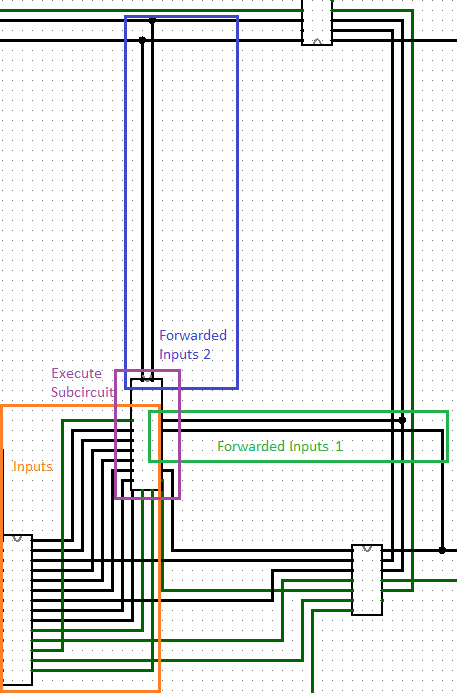
\includegraphics[width=8cm]{ALU.png}
\\
Our Execute stage is all condensed into a big Execute subcircuit, that does the computing, (with additional lower level circuits within the subcircuit) and a smaller subcircuit that aids in stalling. The Execute subcircuit gets its inputs mainly from the ID/EX registers but also from the EX/MEM and MEM/WB registers for use in the forwarding unit. The four outputs of the subcircuit is the main output C, the Write Enable for the Register File (which is conditional in the MOV instructions), a Jump variable, indicating whether or not we branch, and an output for Store functions. 

The Execute subcircuit has many subcircuits of its own. For each of the main inputs, A and B, with respective register addresses rs and rt, there is a forwarding unit that resolves data hazard issues that are present in this Mini-Mips processor. There is a multiplexor for B that chooses between B and the immediate. There are special sections that implement commands whose outputs do not come from the ALU. These commands include SLT, SLTI, SLTIU, and SLTU; MOVZ and MOVN; jumps and branches; and SW and SB. 

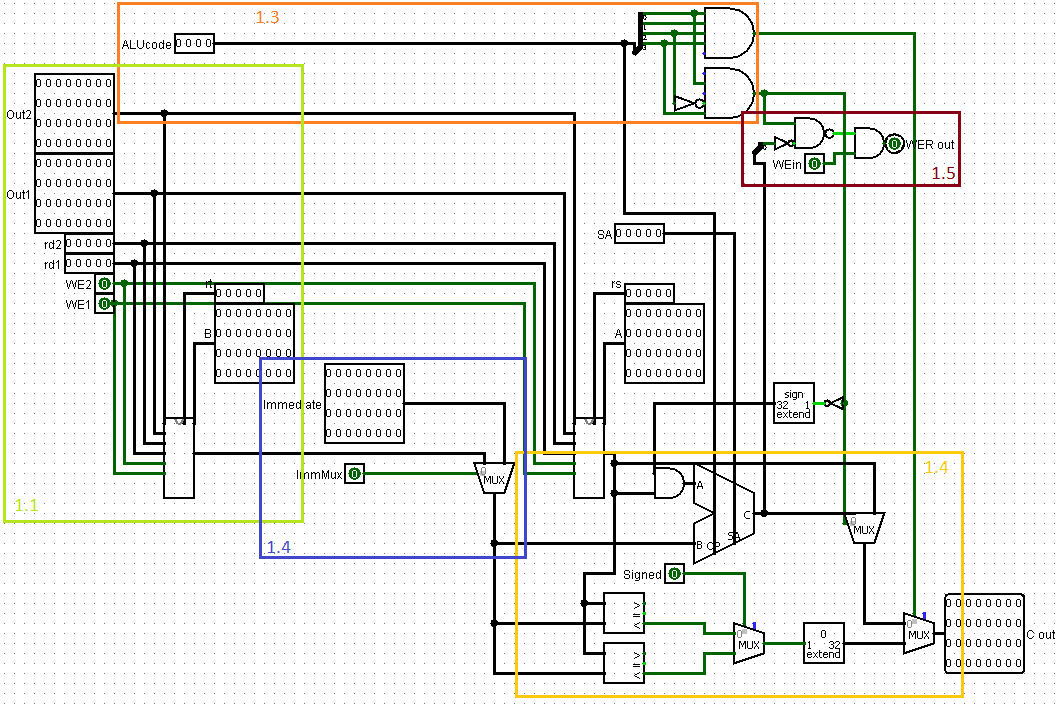
\includegraphics[width=17cm]{EXOVER.png}

\subsubsection{General Purpose ALU}
The ALU (1.3) provides us the output for many of the simpler commands, and also provides us some intermediate outputs for the more specialized commands. Inputs A and B are determined by the specified command, but here we take them as given. We get the Op Code for the ALU as an input (1.1), and the SA is determined in a subcircuit (1.2), depending on whether or not the shift command was variable.  

\subsubsection{Forwarding Unit}
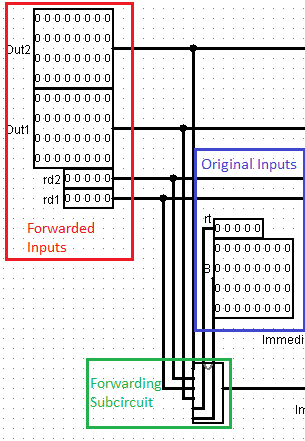
\includegraphics{Forward1.png}
This part of the circuit compares the register address (rs) of a main input (Out0) with the write destinations of the instruction in the next stage (rd1) and the stage after that (rd2). Out1 and Out2 are to be written in those destinations respectively. The write enable bits from those stages need to be included as well. The Forwarding Unit takes these 8 inputs and chooses one of the 3 32-bit outputs Out0, Out1, Out2. Figure 11 shows the layout of the Forwarding Unit and its inputs in the Execute circuit.

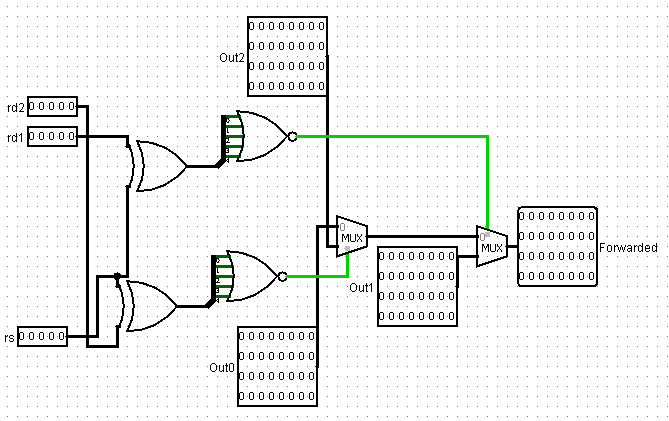
\includegraphics{Forward2.png}
The Forwarding Unit compares the register addresses using an XOR and a NOR gate to get a multiplexor selector, that is, if the register addresses are equal, we get 1, and otherwise 0. Additionally, the current register address must not be 00000. This is ANDed with a write enable bit. This is done for each rs and rd1, and rs and rd2. We first choose between Out0 and Out2 by comparing rs and rd2, then the selected and Out1 by comparing rs and rd1. This process automatically gives Out1 higher priority than Out2; if all of rs, rd1, and rd2 are equal, Out1 will be chosen over Out2. 

Load Forward (2.3) simply computes whether the previous instruction's register address (rd) is the same as the current instruction's rs or rt. This output is used later on in stalling for LW forwarding.

\subsubsection{Immediate Mux}
This section (3.1) determines which of input B or the Immediate become an input for the ALU and the Comparators.

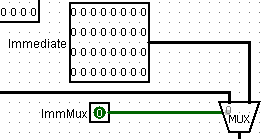
\includegraphics{Immediate.png}
The upper MUX determines the second input of the ALU. The Immediate is already bit extended to 32 bits, and our Decoder gives us a multiplexor selector bit ImmMux that we use here. 

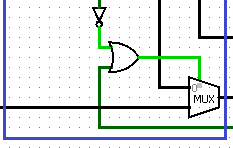
\includegraphics{Immediate2.png}
The lower MUX determines the second input of the Comparators. The difference between this MUX and the upper MUX is that the MUX will choose input B if the command is a Branch command, overriding the ImmMux. 

\subsubsection{MOVN/MOVZ}
MOVN and MOVZ are one of the sets of commands that require special attention. The large AND gate in (4.1) outputs 1 if the ALU Op code is 1x01. Directly right of the AND gate is a subcomponent that disables the Register Write Enable if the ALU returns 0 for the comparison. 

The AND gate in (4.3) replaces input A with a 32-bits of all 0's if the command is MOVN or MOVZ. This is because these commands' conditionals compare against zero. 

Finally the output that is eventually stored if the conditional is true is the input A. Our MUX in (4.2) does exactly that, choosing input A over the ALU output C if the selector bit is 1.

\subsubsection{Comparator}
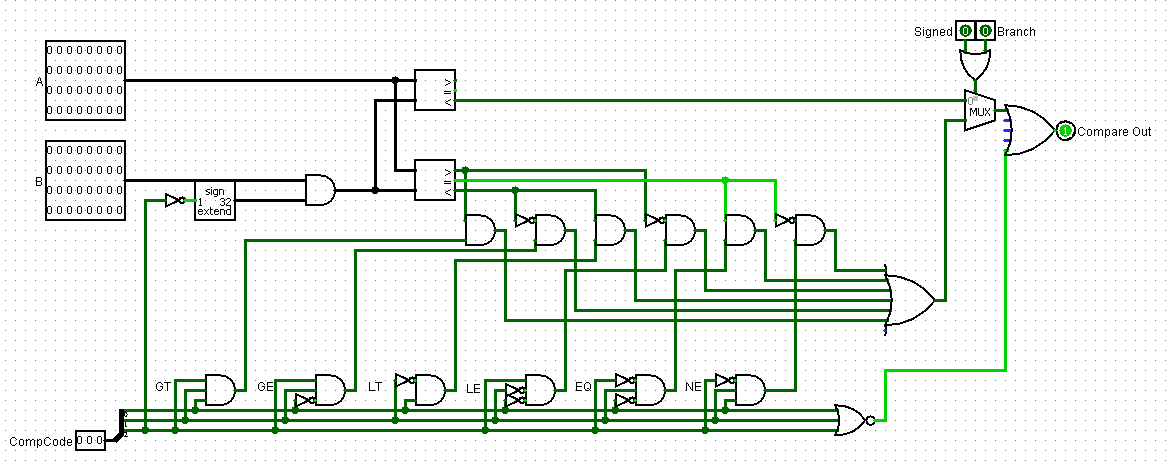
\includegraphics{Compare.png}
The Comparators (5.3) is used for the SLT commands and the branch commands. The upper comparator is unsigned and used for the commands SLTU and SLTIU. 

We use a Comp Code that tells us the exact comparison that we want. 

\begin{tabular}{| c | c |}
\hline 
LEZ & 100 \\ \hline
LTZ & 101 \\ \hline
GEZ & 110 \\ \hline
GTZ & 111 \\ \hline
SLT & 001 \\ \hline
EQ &  010 \\ \hline
NE &  011 \\ \hline
\end{tabular}

\textbf{Design Decisions}
\begin{itemize}
\item
We set all the Comp Codes for comparisons with 0 to 1xx, so we sign extend the negation of the most significant bit of the Comp Code to control the second input to the comparators. 
\item
We represent GE and LE as the negation of LT and GT respectively and that can be seen in the first row of AND gates under the second comparator.
\item
Only 1 of the outputs from the second row of AND gates is 1 for any Comp Code. That means only 1 of the outputs from the first row of AND gates can be 1, and the big OR gate will output 0 unless that specified comparison is true. 
\item
The Comp Code for all other commands is 000, which makes the output of the subcircuit 1 regardless of the inputs. This is required so that Jump instructions always jump.(see (6.3))
\end{itemize}



 The Op code 1111 identifies the command as one of the SLT commands.

\subsubsection{Outputs}
\includegraphics{OUTPUT.png}
The output C out is by default rooted from the output C from the ALU. However, there are 2 multiplexors, M1 and M2, that select for the final output of the subcircuit. M1 corresponds to the commands MOVN and MOVZ; that is, if the ALU Op code is 1x01, the output will be the first main input A (after corrected by the forwarding unit) instead of the output C from the ALU. M3 corresponds to the commands SLT, SLTI, SLTU, SLTIU; that is, if the ALU Op code is 1111, the output will be determined in the section labeled SLT in the figure. 
\begin{itemize}
\item
SLT: We use two comparators to do the SLT commands. For SLTU and SLTIU, we use the upper unsigned comparator, and for SLT and SLTI, we use the lower 2's complement comparator. We choose between the two outputs at multiplexor Y with a bit indicating whether the comparison is signed or not, Signed. Then the 1 bit output is sign extended to 32 bits. 

\item
X: For the MOVN and MOVZ commands, we are comparing B against 0 instead of A. The lower input to the AND gate labeled X is just the original input coming from the Forwarding Unit. The upper input to X is either 32-bits of all 0's if the ALU Op code is 1x01 or all 1's otherwise. The wire leading out of X is therefore all 0's if the command is MOVN or MOVZ, and the original input otherwise.

\end{itemize}
\subsubsection{Write Enable for MOV}
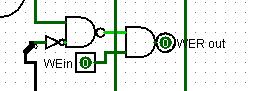
\includegraphics{MOV.png}
The final piece of the circuit deals with the MOVN and MOVZ commands. Since these two only write based on the given condition, we modify the write enable (WE in) if the condition was not met and the command was MOVN or MOVZ to begin with. In our implementation, the lower lead in to the NAND gate is the truth value of the condition, coming from the ALU (negated), and the upper lead in indicates whether or not the command is MOVN or MOVZ. As such, the output of the NAND gate is true if either the command is not MOVx, or if the condition was true. 

\subsection{Correctness Constraints}
\begin{itemize}
\item The correctness of this module depends on the correctness of the inputs that are decoded in the Instruction Decode stage. Therefore, one functional requirement is that the inputs are consistent with the MIPS command given. For instance, WE in (write enable) must be 1 if the command ultimately writes back to the Register File. 
\item The module takes inputs from the Memory and Write Back Stages. Therefore, these stages need to be implemented correctly in order for this stage to be correct.
\item The execute subcircuit in this implementation is only correct for the instructions in Table A, and pseudo correct (set as NOPs) for the instructions in Table B. Only these instructions can be given in the Instruction Fetch Stage.

\end{itemize}

\subsection{Testing}
A large portion of the instructions depend on the correctness of the ALU circuit. Since that is given to us, we assume its correctness. For those instructions, computation is given correct, so we only have to test one case for each, that is, if one case gives us the correct nontrivial output (like 0 or something that could have been an accident), then the data path was correct and all inputs for that instruction should give us a correct output. 

There are 6 functions that are not computed using the ALU: SLT, SLTU, SLTI, SLTIU, MOVN, and MOVZ. For these, we need to check an encompassing set of cases. Since all of these instructions involve a conditional, we check the cases for the conditionals, namely less than, greater than, and equal.

Lastly, we need to test the forwarding unit. We need to test for EX/MEM $\rightarrow$ EX forwarding and MEM/WB $\rightarrow$ EX forwarding. We test with multiple cases to be safe. 
\end{document}